% Cuba 2021--2026 depopulation: English scientific preprint
\documentclass[11pt,a4paper]{article}

\usepackage[margin=2.2cm]{geometry}
\usepackage{times}
\usepackage{amsmath,amssymb}
\usepackage{graphicx}
\usepackage{booktabs}
\usepackage{hyperref}
\usepackage{setspace}
\usepackage{caption}
\usepackage{subcaption}
\usepackage{placeins}
\usepackage{natbib}
\setstretch{1.15}
\captionsetup[subfigure]{font=small,labelfont=bf,skip=4pt}
\captionsetup[figure]{font=small,labelfont=bf,skip=6pt}

\graphicspath{{../../../figures/}}

\title{Scenario audit of Cuba's 2021--2026 population decline}
\author{Yasset P\'erez-Riverol\\
\textit{Independent researcher}\\
\texttt{ypriverol@gmail.com}}
\date{Preprint · 3 August 2026\\[0.35em]
\normalsize Scenario ensembles, an infant-mortality consistency check,\\
an excess-mortality decomposition, and triangulation of independent registers\\[0.4em]
\footnotesize Supplementary figures (life expectancy; provinces):\\
\texttt{cuba-depopulation-2021-2026-supplement.pdf}}

\begin{document}
\maketitle

\begin{abstract}
\textbf{Background.}
Cuba is losing population at one of the fastest peacetime rates in the Western Hemisphere.
No census has been completed since 2012, and the national statistics office (ONEI) revised its published headcount downward by more than one million in a single 2024 revision.
End-2025 published levels still span roughly 8.0--11.0~million.
This paper audits the 2021--2025 headcount decline with transparent scenario ensembles, decomposes migration versus internal demographic change, and reports an end-2026 scenario continuation.

\textbf{Methods.}
We solve the demographic accounting identity under three scenarios---floor, central, upper---each specified by three numbers: end-2021 roll overstatement, a multiplier on ONEI net emigration, and residual death under-registration.
Point figures are closed form and exact by linearity; a reduced Monte Carlo reports prior sensitivity ranges only.
No parameter is informed by a likelihood, so these are scenario values, not estimates, and the ranges are not confidence intervals.
All results are stated against a single base, the official end-2021 stock.
External registers are used as ceilings or soft corroboration; the central scenario is never treated as external validation of itself.
Separately, we decompose the change in annual deaths since 2019 by indirect age standardisation on ONEI age-specific mortality, splitting it into a population-size term, an ageing term, and a residual rate term reported as excess deaths relative to the 2019 age-specific schedule.

\textbf{Results.}
Against the official end-2021 stock of 11.11~million, the gap by end-2025 spans \textbf{1.97--2.79~million} (\textbf{17.8--25.1\%}) across three assumption sets; a null scenario taking ONEI at face value gives 1.68~million (exactly, by construction) and is reported with them.
Two quantities must be kept apart.
Against the \emph{official 2021 stock}, the central scenario's gap is \textbf{2.53~million} (22.8\%)---but 1.68~million of that is decline ONEI itself published, so only \textbf{0.85~million} is this paper's added correction.
Against ONEI's \emph{end-2025} figure of 9.43~million, the central scenario's living population of \textbf{8.58~million} is lower by \textbf{0.85~million}.
That 0.85~million is the paper's actual claim; the 2.53~million is the two combined.
A null scenario ($U_0{=}0$, $M{=}1$, $D_{\mathrm{fac}}{=}1$) reproduces ONEI's published figure exactly---necessarily so, since $R$ is defined as the residual that closes the identity---and is reported alongside the three assumption sets so the span does not exclude the official series by construction.
About \textbf{92\%} of that gap is emigration, counting both the 2022--2025 flow and the pre-2021 backlog still on the roll.
The end-2026 continuation places the central scenario near \textbf{8.29~million}.
Cuba registered 27{,}100 more deaths in 2025 than in 2019, or some 31{,}300 once estimated unregistered deaths are added, while the central scenario's stock is about 2~million smaller.
Age standardisation separates two upward forces of comparable size---about \textbf{22{,}400} additional deaths per year from an older population and about \textbf{28{,}500} per year of excess against the 2019 schedule (prior sensitivity range 18{,}600--38{,}200)---against roughly 19{,}400 fewer deaths per year from the smaller population.
Excluding the 2021 pandemic wave, the excess total over 2022--2025 is $\sim$\textbf{74{,}800} (47{,}000--103{,}000), conditional on a flat 2019 anchor; the choice of counterfactual moves it across 45{,}200--103{,}300, which is the dominant uncertainty and is not inside that range.

\textbf{Conclusions.}
Depopulation is predominantly migratory in the headcount, reinforced by collapsing births, elevated mortality, and accelerated ageing.
Against the official 2021 stock the end-2026 gap approaches one in four; because a single base is used throughout, this is the same quantity as the headline, not a second definition.
Mortality is a small share of headcount loss but a large absolute toll: it is separately measurable, roughly half of it is not explained by ageing, and it is still rising.
\end{abstract}

\noindent\textbf{Keywords:} Cuba; demography; emigration; natural decrease; infant mortality; fertility; ageing; statistical data quality.

\section{Introduction}

Counting Cubans has become contested.
The last completed census was in 2012; the census planned for 2022 has been repeatedly postponed and is now promised for 2026~\citep{onei_census}.
Without a census, published population depends on projections and a lagging migration register~\citep{preston2001,un_wpp}.
In July 2024, ONEI reported an ``effective population'' of 10{,}055{,}968 at end-2023 (about one million below prior published levels), then 9{,}748{,}007 (end-2024) and 9{,}434{,}593 (end-2025)~\citep{onei_revision,onei_2025}.

Three incompatible series coexist (Figure~\ref{fig:pop}):
the United Nations World Population Prospects path near 10.9~million (still assuming net emigration of order $2\times10^4$ per year)~\citep{un_wpp,eclac2022};
ONEI's revised official series (9.43~million at end-2025);
and independent studies placing the living population nearer 8.0--8.6~million~\citep{albizu2023,albizu2024}.
Almost three million people separate the extremes.
This paper presents a scenario audit of the 2021--2025 headcount decline with transparent prior ensembles, decomposes migratory and internal components, compares official migration accounting with destination registers, and reports an end-2026 scenario continuation.

Cuba's fertility transition was already among Latin America's earliest and deepest~\citep{diazbriquets1982,hollerbach1984,diazbriquets2014}, so below-replacement fertility is not new.
What is new is the \emph{speed} of headcount loss under combined emigration and natural decrease, in a regional context where Latin America and the Caribbean still grow overall~\citep{eclac2022,un_wpp}.
Comparable peacetime contractions elsewhere have been driven primarily by emigration (e.g.\ Venezuela)~\citep{coleman2006,pagegarcia2020}.

\textbf{Central thesis.}
The headcount loss is mostly emigration, but a second ``internal'' engine (birth decline, excess mortality, and ageing) would sustain contraction even if emigration slowed~\citep{lee2014,lesthaeghe2010}.
The two engines are not independent: selective exit of working-age adults and women of reproductive age causes much of the fertility decline, so many ``births that do not occur'' are a delayed migratory effect~\citep{bongaarts2009,diazbriquets2014}.

\section{Methods}

The balancing equation is the standard demographic accounting identity~\citep{preston2001}.
Registered ONEI aggregates over 2022--2025 are fixed anchors~\citep{onei_2025}. Their provenance is uneven: 2019--2022 vital counts are in the ONEI tables we ship, 2023 deaths are independently corroborated by Cuba's WHO submission, but the 2024 births and deaths (71{,}374 and 128{,}098) appear in no table available to us and rest on state reporting. The 2024 death total feeds the 2024 excess figure and every cumulative window, and is the weakest link in the series.
births $B^{\mathrm{reg}}=325{,}233$, deaths $D^{\mathrm{reg}}=502{,}149$,
and identity-consistent net emigration $R=1{,}501{,}706$.
Official end-2021 population is $P^{\mathrm{off}}_{2021}=11{,}113{,}215$.
Each Monte Carlo draw samples latent corrections and applies
\begin{align}
P_{2021} &= P^{\mathrm{off}}_{2021} - U_0, \\
D &= D^{\mathrm{reg}}\,D_{\mathrm{fac}} \;\;(+\;\text{optional epidemic pulse in B/C}), \\
M_{\mathrm{net}} &= R\,M, \\
\Delta &= (D - B) + M_{\mathrm{net}}, \\
P_{2025} &= P_{2021} - \Delta,
\end{align}
where $U_0$ is end-2021 baseline overstatement (people already effectively abroad but still on the roll),
$M\ge 1$ scales ONEI net emigration, and $D_{\mathrm{fac}}\ge 1$ scales registered deaths.
Loss is reported on a single base: the \emph{official} end-2021 stock.
The gap it defines has three additive parts---baseline overstatement $U_0$, net emigration $R\,M$, and natural decrease---so no second ``corrected base'' percentage is needed.

Each scenario is three numbers, and the point figure is the arithmetic above evaluated at their prior means, which is exact because the identity is linear in all three.
We verified that this is all the simulation was doing: the closed form and a Monte Carlo over the same margins agree to within a few hundred people (1{,}117 in the upper scenario), i.e.\ to sampling noise.
The copula has therefore been removed---it moved the median by $\sim$2{,}200 people and only widened a within-scenario band that is not our primary uncertainty statement.
A reduced draw ($N=2\times10^5$, independent margins) is retained solely to report that band, which remains a \emph{prior-predictive} spread under fixed Beta margins, not sampling error.
The \textbf{across-scenario envelope} is the primary uncertainty statement~\citep{repo,modeld}.

We define three scenarios, each earning its place.
\textbf{Conservative} adds a modest correction. It is \emph{not} an ONEI-consistent lower bound: its mean $M$ is 1.089, i.e.\ 9\% more emigration than ONEI reports. The zero-correction case is the null scenario.
\textbf{Central} raises the migration prior above ONEI and caps residual death under-registration at 9\%---just above the 7.5\% the register itself shed in 2022 without explanation.
\textbf{Upper} defines the top of the envelope.
Earlier versions carried five prior sets; two have been retired.
A crisis-adjusted variant landed within 0.02~million of the central scenario---the same scenario with different dials---and a vital-reconstruction companion built on a hand-weighted deterioration index has been superseded by the attributable-mortality decomposition below, which estimates the same quantity from observed age-specific data rather than from a dimensionless score.
These are \textbf{scenarios} (prior narratives), not identified estimators of a unique living population.
ONEI's 2023--2024 revisions already absorbed a large lagged stock, so scaling revised $R$ by $M>1$ \emph{and} subtracting a large $U_0$ can double-count the same outdated-register defect; we therefore always report the floor beside the central path and treat $U_0+(M-1)R$ as constrained by destination floors plus documented lag.

\begin{table}[ht]
\centering
\caption{Central-scenario specification. Three margins, no dependence structure.
Beta scales: $U_0\in[0,700{,}000]$, $M\in[1,1.72]$, $D_{\mathrm{fac}}\in[1,1.09]$.
Birth noise independent $B=B^{\mathrm{reg}}\mathcal{N}(1,0.01^2)$.
The point figure uses the prior means of these three margins.}
\label{tab:priors}
\begin{tabular}{llp{6.2cm}}
\toprule
Symbol & Margin & Interpretation \\
\midrule
$U_0$ & $700{,}000\times\mathrm{Beta}(2.0,2.4)$ & End-2021 roll overstatement \\
$M$ & $1+0.72\times\mathrm{Beta}(2.2,2.4)$ & Multiplier on ONEI net emigration $R$ \\
$D_{\mathrm{fac}}$ & $1+0.09\times\mathrm{Beta}(1.8,3.2)$ & Residual death under-registration (at-home elderly channel) \\
\bottomrule
\end{tabular}
\end{table}

Infant mortality rose from 5.0 to 9.9 per thousand live births (2019--2025), a $\sim$98\% increase in the \emph{rate}. The 2025 value is a reported figure and is not in any ONEI table available to us.
Most of that is the denominator: infant \emph{deaths} rose from 552 (observed, ONEI 3.16) to $\sim$674 (derived), about 22\%, while live births fell 38\%.
Both figures matter and only reporting the rate overstates the signal.
Infant deaths are comparatively hard to hide (hospital occurrence; international scrutiny), so the infant rate is often treated as a high-integrity sentinel of health-system \emph{stress}. Two caveats temper that: the 2025 value is press-reported and absent from the ONEI tables available to us, and there is a literature questioning late-fetal/early-neonatal classification at the viability margin in Cuba~\citep{berdine2018}, so part of any rise may be relaxation of classification practice rather than deterioration.
Over the same period the registered crude death rate rose from 9.7 to 14.2 per thousand ($\sim$46\%).
Both moved sharply upward together, which is what a deteriorating system with an intact death register looks like; a register concealing deaths at scale would show the sentinel rising while all-cause mortality stayed flat.
Earlier versions converted this into a log-elasticity calibrated on Venezuela and reported a predicted CDR rise.
That step has been removed: it rested on two numbers from one country with no uncertainty attached, and the conclusion---no signature of large-scale concealment---follows from the co-movement without it.
Residual under-registration in the central scenario is accordingly limited to a small at-home elderly channel (central $\sim$3\%, cap 9\%)~\citep{modeld}.

Mortality is treated as a separate estimand from the headcount, and the question it answers is separate too: how many Cubans are dying because the health system has deteriorated, as opposed to because the resident population is older?
A crude-rate baseline cannot answer this, because it charges the entire ageing shift---from 20.4\% aged 60+ in 2019 to roughly 25--27\% in 2025---to the crisis.
We therefore replace the crude bridge used in earlier versions of this work with indirect age standardisation~\citep{preston2001}.

Let $m^{2019}_a$ be age-specific death rates in 2019 from ONEI table 3.15, over the groups $a\in\{0\text{--}14,\,15\text{--}59,\,60\text{--}64,\,65+\}$---the finest set the deaths table shares with ONEI table 3.3, which publishes mid-year population by age annually.
Splitting 60+ matters: the 1960s birth cohort is now entering at 60--64, so the elderly group is becoming \emph{younger} (60--64 rose from 25.7\% of the 60+ population in 2019 to 27.9\% in 2022), and a single open-ended 60+ group would misread that composition shift as rising mortality.
Expected deaths in year $t$ under an unchanged 2019 health system are $E_t=\sum_a m^{2019}_a P_{a,t}$, and the change in annual deaths since 2019 decomposes exactly into
\begin{align}
\text{size} &= (P_t-P_{2019})\,\mathrm{CDR}_{2019}/1000, \\
\text{ageing} &= \textstyle\sum_a m^{2019}_a (P_{a,t}-P_{a,2019})/1000 - \text{size}, \\
\text{rate} &= D_t\,D_{\mathrm{fac}} - E_t,
\end{align}
with $D_t D_{\mathrm{fac}} - D_{2019} = \text{size}+\text{ageing}+\text{rate}$.
This is a Kitagawa-type decomposition applied to a death \emph{count} rather than to a crude-rate difference; the size term is the count analogue of holding exposure fixed~\citep{kitagawa1955}.
The rate term is \emph{excess deaths relative to the 2019 age-specific schedule}.
We deliberately do not call it ``attributable to health-system deterioration''.
The same formula applied to 2021 returns $\sim$61{,}900, which is a pandemic, not a health system; a residual against a fixed schedule absorbs pandemic and post-acute mortality, coding drift, mortality displacement, health-selective emigration, and denominator error without discriminating among them.
Attribution would require an identified exposure, cause-of-death evidence consistent with the mechanism, and quantitative exclusion of competitors---none of which we have.

The decomposition is far less denominator-sensitive than the crude bridge it replaces.
In 2019, 82\% of Cuban deaths occurred at ages 60+, while emigration is $\sim$77\% aged 15--59.
We therefore hold the elderly \emph{count} approximately fixed across stock scenarios, so that under the central-scenario stock the same elderly people sit on a smaller total and the 60+ share rises to $\sim$29\% (against $\sim$26\% officially).
That $\sim$29\% is an assumption of this decomposition, not an observation, and it is deliberately conservative: because 8\% of emigrants are themselves aged 60+, holding the count fixed slightly overstates expected deaths and so understates the attributable residual.
Its consequence is that $E_t$ barely changes between the official ($\sim$9.4~M) and central-scenario ($\sim$8.6~M) stocks, whereas a crude rate applied to the smaller stock mechanically inflates the residual.
Age structure is \emph{observed} for 2019--2022 and cohort-projected for 2023--2026 from the observed 2022 structure, with entrants from the 55--59 cohort, exits at the 2019 schedule, and elderly emigration at the 8\% share of emigrants aged 60+ (an expert prior, not a measurement). Ages 40--59 receive no emigration or mortality depletion and $U_0$ is not removed from the 2022 age structure; both omissions inflate the projected elderly stock, raise $E_t$, and therefore \emph{lower} the excess we report, by roughly 1{,}000 deaths in 2025.
We never derive the elderly count as (age share $\times$ official total): the official total absorbs ONEI's 2023 register catch-up in a single step, and multiplying that step by an age share deletes elderly residents who never emigrated.
We propagate four sources of uncertainty over $N=2\times10^5$ draws: 2\% noise on the 2019 schedule; a symmetric $\mathcal{N}(0,0.03)$ residual drift for within-65+ composition after 2022; the central-scenario $D_{\mathrm{fac}}$ prior for unregistered deaths; and a 50/50 mixture over official and central-scenario population paths, with a projection error growing 1.5\% per year beyond 2022.
Systematic parameters are drawn once and reused in every year, so cumulative windows propagate correlated rather than independent error.
The identity above closes exactly in every draw because the 2019 reference uses the same perturbed rates as the target year.
Because $D_{\mathrm{fac}}$ is shared with the central scenario, the excess estimate and the headcount scenario are not independent.
One further choice must be stated: $D_{\mathrm{fac}}$ lifts the target years but not the 2019 anchor, so it enters as a \emph{deterioration in registration completeness since 2019} rather than as a constant level. That is the reading we intend---a crisis-induced at-home elderly channel that did not exist in 2019 genuinely produces excess deaths---but it raises the result. Applying $D_{\mathrm{fac}}$ symmetrically to the anchor gives 24{,}900 for 2025 and 60{,}600 for 2022--2025, about 13\% and 18\% below the headline.
Earlier versions also carried a crude registered-excess comparator on a linear-drift counterfactual. It has been dropped: it did not reproduce from the stated formula, its drift was below Cuba's own observed pre-crisis crude drift, and it served no argument the age-standardised decomposition does not serve better~\citep{karlinsky2021,msemburi2023,kishore2018}.

Published population levels are grouped by information content (Figure~\ref{fig:tri}).
Ceilings that do not purge emigrants include the UN World Population Prospects, the MINSAP denominator, and the electoral roll (soft upper bounds only).
The official ONEI revised headcount is 9.43~M at end-2025.
Exit-correcting or independent constructs include housing$\times$occupancy ($\sim$8.7~M; fragile occupancy scalar) and Albizu-Campos 2023/2024 (8.0--8.6~M; methods that share migration-critique assumptions with this paper).
The central scenario (8.58~M) is the study estimand and is \emph{not} external validation of itself; agreement with Albizu/housing is partly shared-prior echo, while ceilings bound the upside.
The soft band from exit-correcting sources is near 8.0--8.9~million.

The settled-concept destination floor (Table~\ref{tab:bridge}) comprises United States $\sim$800{,}000 (administrative/CBP-pipeline statuses, \emph{not} ACS stock), non-U.S.\ total $\sim$250{,}000 (Spain $\sim$135{,}000 + Uruguay $\sim$35{,}000 + rest $\sim$80{,}000), and floor $\sim$1.05~million~\citep{destinations,pew_cuban}.
ACS Cuban-born stock rose by only $\sim$335{,}000 from 2019--2024---a lower stock-change floor that must not be silently equated with the 800{,}000 administrative figure.
Encounter counts and nationality applications are separate concepts and are never added into the settled floor~\citep{cbp_encounters}.

\begin{table}[ht]
\centering
\caption{Bridge from settled destination floor toward scenario migration engines.
Only the floor is ledger-like; later rows are residuals or priors, not destination microdata.}
\label{tab:bridge}
\begin{tabular}{lrl}
\toprule
Concept & Approx.\ count & Role \\
\midrule
Settled destinations floor (US admin + non-US) & 1.05~M & Lower bound (settled concept) \\
U.S.\ ACS Cuban-born rise 2019--24 (not settled) & $\sim$0.34~M & Stock-change floor; do not add \\
Unquantified gap toward ONEI $R$ & $\to\sim$1.5~M & Residual, not validated persons \\
ONEI identity-consistent net $R$ (2022--25) & 1.50~M & Official flow after revision \\
Albizu-Campos--type net & $\sim$1.8~M & Independent upper narrative \\
Central-scenario median $R\times M$ & $\sim$2.0~M & Prior-driven scenario engine \\
U.S.\ encounters 2022--2024 (not settled) & $\sim$0.85~M & Events; do not add to floor \\
Spain nationality applications & $\sim$0.30~M & Many applicants still in Cuba \\
\bottomrule
\end{tabular}
\end{table}

Destination data do \emph{not} identify the central scenario's $\sim$2.0~million net emigration; they support a large floor and leave the 1.05$\to$2.0 path as soft gap-filling plus a migration prior.
If true net emigration were nearer 1.5 than 2.0~million, living population would sit toward $\sim$9.1 rather than $\sim$8.6~million; cumulative loss would remain large and emigration would still dominate absolute loss under every scenario in Table~\ref{tab:models}.
Conditional on end-2025 draws, the end-2026 scenario continuation uses births centered at 65{,}682 ($\mathcal{N}$ noise 3\%),
deaths centered at $1.04\times 136{,}214$ times the same $D_{\mathrm{fac}}$,
and a three-regime net emigration mixture with probabilities $(0.35,0.35,0.30)$ on centers $(150{,}000,\;210{,}000,\;300{,}000)$ plus 15\% log-scale noise.
The $\sim$4\% death lift and regime weights are scenario assumptions, not a validated forecast.
Paths to $\sim$7~million by 2030 in Figure~\ref{fig:pop} are \textbf{illustrative trend scenarios} (visually the post-2026 segment); they are not probabilistic forecasts.

\section{Results}

\begin{table}[ht]
\centering
\small
\caption{Headline quantities by claim. Bands are 90\% prior-predictive under the
stated margins, not sampling error. ``Scenario'' marks a quantity that depends on
an assumption rather than an observation.}
\label{tab:headline}
\begin{tabular}{llrl}
\toprule
Claim & Quantity & Value & Status \\
\midrule
\multicolumn{4}{l}{\textit{Migration}} \\
& Settled destination floor, documented & 1.05~M & lower bound \\
& ONEI identity-consistent net, 2022--25 & 1.50~M & official \\
& Central-scenario migration engine & $\sim$2.0~M & prior \\
& Emigration share of the 2022--25 flow (central) & $\sim$91\% & scenario \\
& ONEI declared net migration, 2021 / 2022 & $+$169 / $+$991 & official \\
& US-recorded Cuban arrivals, 2021 / 2022 & 54{,}818 / 313{,}506 & external \\
& High-severity consistency failures & 7 of 18 & audit \\
\midrule
\multicolumn{4}{l}{\textit{Health-system deterioration}} \\
& Registered deaths, 2025 & 136{,}214 & official \\
& Expected at 2019 rates, 2025 age structure & 112{,}100 & derived \\
& Excess vs 2019 schedule, 2025 & 28{,}500 [18{,}600--38{,}200] & scenario value \\
& Excess, 2022--2025 (post-pandemic) & 74{,}800 [47{,}000--103{,}000] & scenario value \\
& \quad under alternative counterfactuals & 45{,}200--103{,}300 & sensitivity \\
& \quad on the pre-revision 2022 total & $\sim$84{,}100 & sensitivity \\
& Explained by ageing alone, 2025 & 22{,}400 & derived \\
& Population-size effect, 2025 & $-$19{,}400 & derived \\
& Standardised mortality ratio vs 2019, 2025 & 1.215 & derived \\
& Share of crude death rate that is age structure (2019) & 40.8\% & derived \\
& Documented 2022 register removal & 8{,}951 (7.5\%) & official \\
\midrule
\multicolumn{4}{l}{\textit{Projected population}} \\
& Gap vs official 2021, across assumption sets & 1.97--2.79~M & scenario span \\
& \quad of which ONEI's own published decline & 1.68~M & official \\
& \quad this paper's added correction (central) & 0.85~M & scenario value \\
& Living population end-2025 (central) & 8.58~M & scenario \\
& Gap, central scenario & 2.53~M (22.8\%) & scenario \\
& ONEI official end-2025 & 9.43~M & official \\
& Living population end-2026 (central) & 8.29~M & scenario \\
& Emigration share incl.\ pre-2021 backlog (central) & $\sim$92\% & scenario \\
\bottomrule
\end{tabular}
\end{table}

\subsection{Migration}


Table~\ref{tab:bridge} separates settled counts from encounters, ACS stock change, and nationality applications.
The settled floor ($\sim$1.05~M) confirms that emigration is large while remaining a lower bound.
Closing the gap to ONEI's $\sim$1.5~million is an unquantified residual; the central scenario's $\sim$2.0~million is a prior on $R$, not destination identification.
If true net is nearer 1.5 than 2.0~million, living population sits toward the high end of our band ($\sim$9.1 rather than 8.6~M).
Emigration still dominates absolute loss under every scenario in Table~\ref{tab:models}.

ONEI's own numbers contradict the destination registers before any model is applied (Figure~\ref{fig:mig}).
For 2021 and 2022 ONEI declares net \emph{arrivals} of $+$169 and $+$991, while the United States alone recorded 54{,}818 and 313{,}506 Cuban arrivals in those years.
A systematic pass over the published series (\texttt{scripts/consistency\_model.py}) returns 18 tests, of which 7 fail at high severity: two of them (T2, the four conflicting official 2022--2023 death totals; and T4, the 2023 rate-versus-denominator contradiction) use only official sources, so those inconsistencies are internal to ONEI's own published series.
The 2023 series shows a single-year population drop of 1{,}033{,}543 against a natural decrease of 27{,}347, implying a migration component of 1{,}006{,}196---more than double any documented annual outflow, and best read as a backlog correction booked as one year's flow.
The published 2023 crude death rate of 11.5 per thousand implies a mid-year population of 10.24~million against 10.57~million in the published series, a gap of 334{,}000; the two figures cannot both be correct.

Cause-specific standardisation is possible for 2021--2022 only, using Cuba's own ICD-10 submission to WHO over ONEI 3.3 denominators, and we report it because one result cuts against the framing above.
Cuba's crude cause-specific rates run about 1.9 times their age-standardised values, so comparisons of Cuban crude rates against regional standardised rates---common in public commentary---overstate Cuba's position roughly twofold.
On a like-for-like basis Cuba's ischaemic-heart mortality is \emph{below} the regional figure often quoted against it (age-standardised 87.2 per 100{,}000 against $\sim$105), and its cerebrovascular rate is about 1.5 times the regional baseline rather than the 27-fold figure obtained by comparing a Cuban 75+ age-specific rate with an all-ages regional one.
Standardised diabetes mortality also \emph{fell} 36\% and neoplasms 6\% between 2021 and 2022.
We do not read the falls as improvement---2021 is a pandemic peak, and diagnosis-dependent causes become less visible when diagnostic capacity fails---but we decline to read them as corroboration either, and note that ill-defined-cause shares (R00--R99, 0.87--0.98\%) are stable across the period, which is evidence \emph{against} certification deterioration.
Cause-specific work cannot be extended past 2022 because ONEI 3.3 denominators stop there, which is also why no cause enters the excess estimate.

About \textbf{77\%} of emigrants are aged 15--59 and the median leaver is about 30 years old (Figure~\ref{fig:mig}); both are expert priors synthesised from the Albizu-Campos reports rather than measurements, as is the 8\% elderly share that drives elderly emigration in the projection.
Among those remaining, the reported official share aged 60+ is about 26.7\% (median age $\sim$45); note that ONEI table 3.12 projects 25.0\% for 2025, and 26.7\% is a reported figure we cannot reproduce from the published tables---neither is a central-scenario-consistent stock.
Exit hollows the centre of the pyramid and removes those who would have children~\citep{coleman2006,lee2014}.
The flow is majority female~\citep{albizu2023} and concentrated at working ages (Figure~\ref{fig:mig}).
Subnational outflow is uneven: ONEI-reported Havana net emigration is about \textbf{$-$33 per 1{,}000} in 2025 (provincial ranks more reliable than levels if national migration accounting is biased; map in the supplement).
Selectivity of exit and the ageing it produces are two views of the same process (Figure~\ref{fig:mig}).


\begin{figure}[!htbp]
\centering

\includegraphics[width=\linewidth]{f15_migracion.png}
\caption{The migration claim, in three panels.
Left: age composition of emigrants against remaining residents---the exodus is selective.
Centre: net migration ONEI declares against Cubans other countries recorded arriving; ONEI reports net \emph{arrivals} in 2021 and 2022.
Right: the bridge from a documented settled floor to the central scenario's migration engine. Only the first bar is ledger-like.
The working-age hollowing in the left panel is what drives the ageing term in Figure~\ref{fig:attrib}.}
\label{fig:mig}
\end{figure}
\FloatBarrier

\subsection{Internal demographic engine and health-system deterioration}

Reducing the crisis to emigration alone is incomplete: emigration can reverse, but missing births and an aged residual population cannot.
A useful distinction is \textbf{realized loss} (exit-dominated) versus \textbf{future inertia} (natural decrease increasingly important).
In 2019 the natural balance was still slightly positive ($+$636); in 2025 deaths exceeded births by \textbf{68{,}150} (68{,}064 births versus 136{,}214 deaths; Figure~\ref{fig:scissors}).
That 2025 deficit matches the 2021 COVID peak without a pandemic: natural decrease is now structural.
The total fertility rate fell to 1.29 children per woman in 2025, the lowest since 1958 and well below replacement (2.1)~\citep{diazbriquets2014,bongaarts2009,lesthaeghe2010}.
Emigration removes young women (majority-female flow) and those who remain defer births under scarcity.
Births fell 38\% (from $\sim$110{,}000 in 2019 to 68{,}000 in 2025).
A back-of-envelope split into ``half fewer women / half lower TFR'' is \emph{illustrative only}: ONEI TFR denominators may themselves be inflated by absent women, which would overstate the rate half; a formal exposure--ASFR decomposition is not claimed here.
The reported share aged 60+ moves from 20.4\% (2019) to 26.7\% (2025)---a figure we noted above is not reproducible from the published tables, against ONEI 3.12's own projection of 25.0\%---and toward 33\% by 2035 under a larger living stock than the central scenario~\citep{onei_2025,lee2014}.
Under a smaller, youth-depleted stock the elderly share would be higher; any $\sim$29\% / $\sim$40\% figures in companion graphics are \textbf{illustrative sketches}, not cohort-component estimates.
Median age reached \textbf{45} years in 2025 on official reporting (Figure~\ref{fig:aging}).

\begin{figure}[!htbp]
\centering
\begin{subfigure}[t]{0.495\linewidth}
\centering
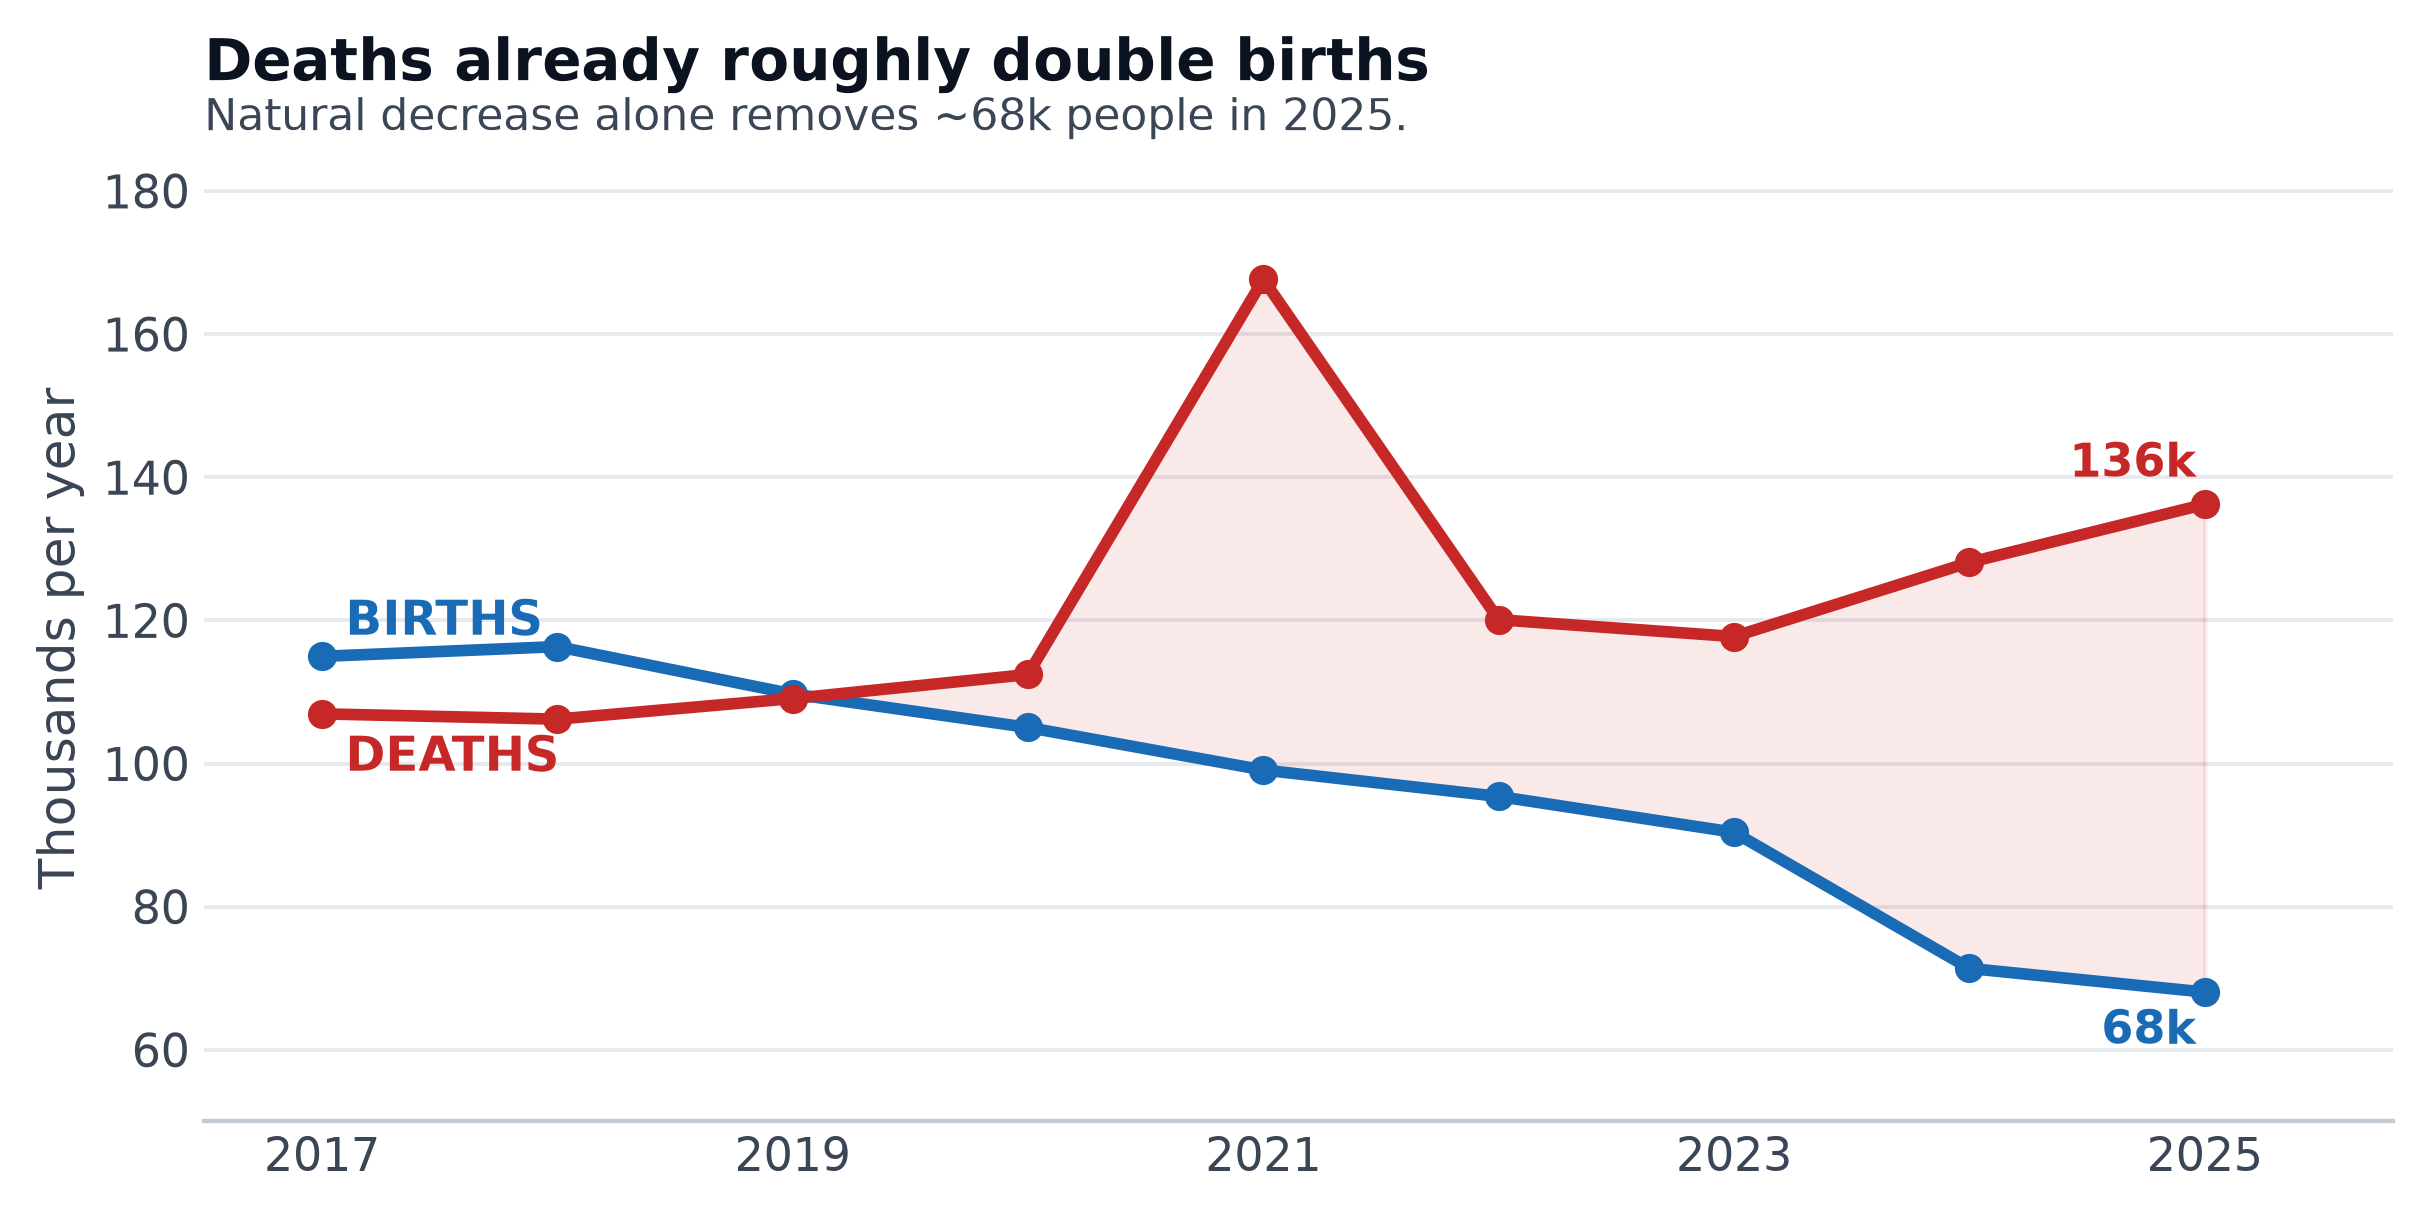
\includegraphics[width=\linewidth]{f2_tijera.png}
\caption{Births versus deaths (``scissors''): deaths roughly double births by 2025.}
\label{fig:scissors}
\end{subfigure}\hfill
\begin{subfigure}[t]{0.495\linewidth}
\centering
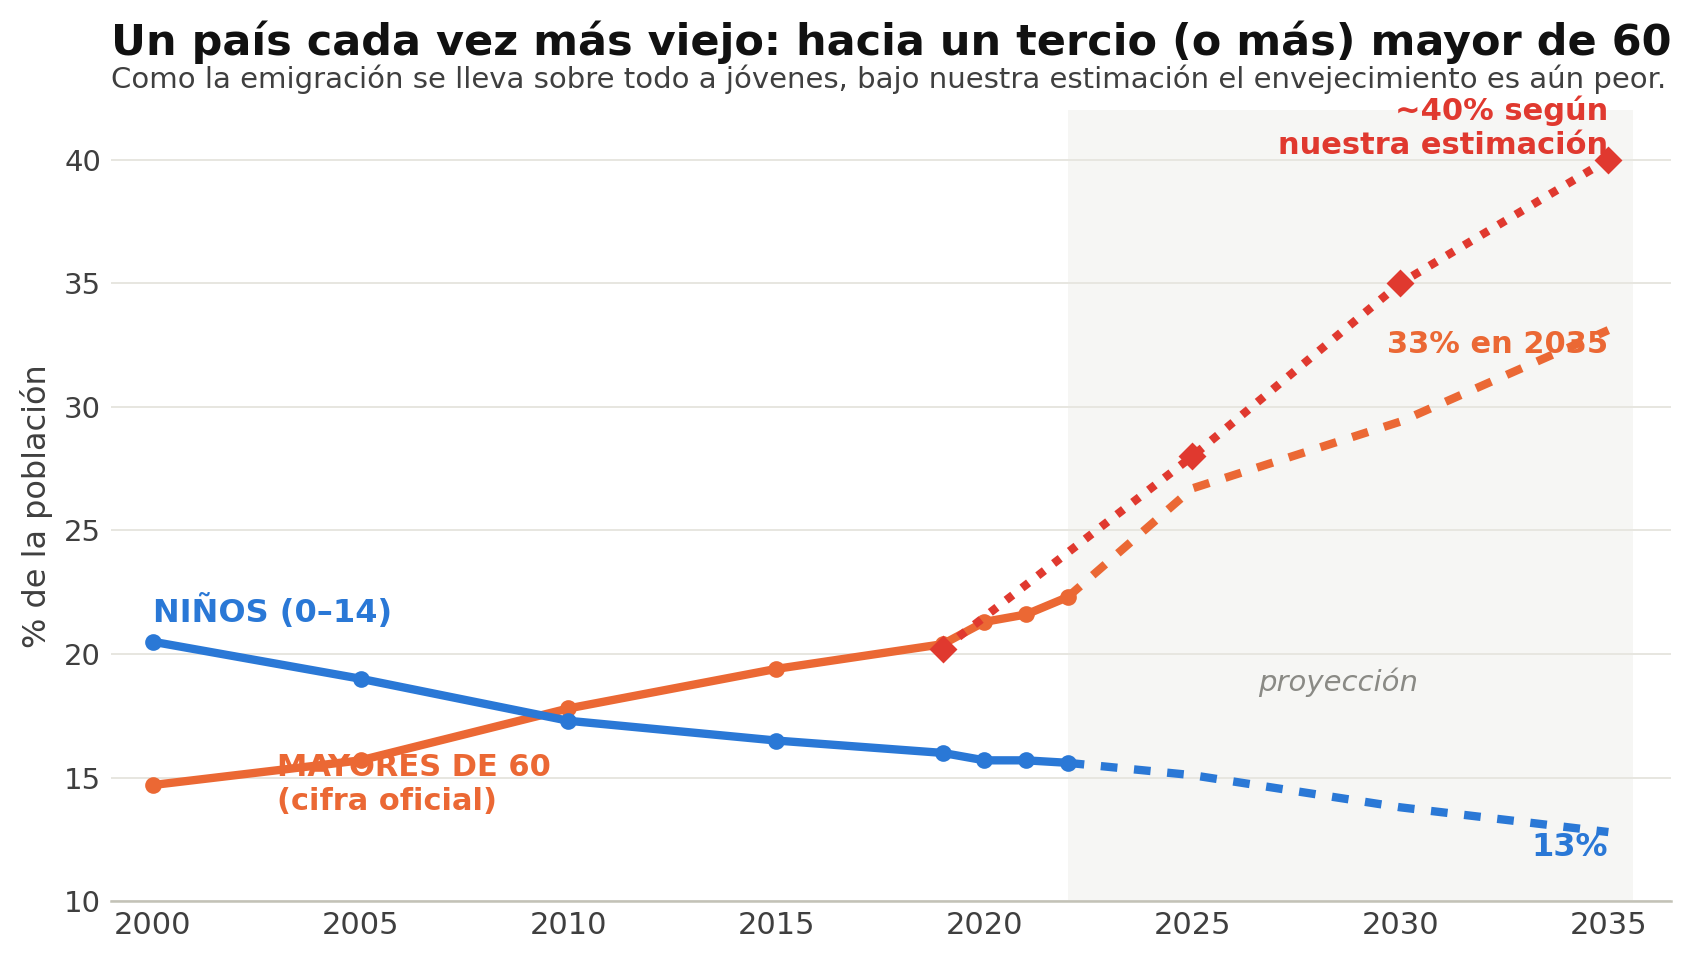
\includegraphics[width=\linewidth]{f4_envejece.png}
\caption{Accelerated ageing as working-age adults leave (official structure).}
\label{fig:aging}
\end{subfigure}
\caption{Internal demographic engine: natural decrease and accelerated ageing.}
\label{fig:internal}
\end{figure}

Official life expectancy at birth peaked in 2011--13 (78.5 years) and fell to 77.7 in 2018--20; an independent 2021 estimate places it near 71 years~\citep{albizu2023,bronnum2023}.
That decline is large relative to COVID-era international losses~\citep{aburto2022,msemburi2023}; LE re-expresses mortality rather than independently corroborating the central scenario (series in the supplement).
Infant deaths rose from 461 (2018) to 715 (2022); the rate reached 9.9 per thousand in 2025 ($+$98\% since 2019).

The mortality decomposition answers the ageing-versus-collapse question directly (Figure~\ref{fig:attrib}).
Cuba registered 136{,}214 deaths in 2025 against 109{,}080 in 2019---27{,}134 more, or some 31{,}300 once estimated unregistered deaths are added---while the central scenario's stock is about 2~million smaller (the official series falls by 1.76~million over the same span).
The 60+ population meanwhile rose from 2.31~million (2019, observed) to a projected 2.60~million in 2025.
Three terms account for that rise (medians are not additive, so they sum to 31{,}500 rather than 31{,}300).
A resident population smaller by $\sim$2~million should have reduced annual deaths by about \textbf{19{,}400}; ageing added about \textbf{22{,}400}; and the residual excess against the 2019 schedule is about \textbf{28{,}500} per year (prior sensitivity range 18{,}600--38{,}200), or $\sim$297 per 100{,}000 on the official stock.
The two upward terms are of comparable magnitude ($\sim$44\% and $\sim$56\% of the gross increase); neither alone accounts for the rise, and together they exceed it because the shrinking population pulls the other way.
The crude bridge reported in earlier versions of this work charged the whole ageing shift to the crisis and overstated the collapse component: $\sim$77{,}000 for 2024--2025 combined against \textbf{50{,}100} (32{,}600--67{,}500) here.

The time profile separates two distinct episodes.
Excess deaths against the 2019 schedule were about 5{,}400 in 2020, peaked at $\sim$61{,}900 in the 2021 COVID-19 wave, fell back to $\sim$12{,}800 (2022) and $\sim$11{,}900 (2023), and then roughly doubled to $\sim$21{,}600 (2024) and $\sim$28{,}500 (2025).
The 2022--2023 trough separates the pandemic wave from the later rise, so the 2024--2025 increase is not a continuation of the 2021 peak; it coincides with the blackout, fuel, medicine, and arbovirus crises, though the residual cannot by itself exclude post-acute COVID-19 mortality or coding drift as contributors.
Excluding 2021 entirely, the 2022--2025 excess total is $\sim$\textbf{74{,}800} (47{,}000--103{,}000); including it, 2020--2025 gives $\sim$142{,}100 (105{,}400--180{,}500).
A 2026 scenario continuation reaches $\sim$32{,}300 (20{,}000--44{,}200), but that figure inherits the assumed $+$4\% death continuation and is not an observation.
The dominant uncertainty is not inside the simulation but in the choice of counterfactual, and it is not in the range above.
Holding 2019 mortality flat is an assumption, and we fit the pre-crisis trend rather than assert it. The result is that \textbf{the trend is not identifiable}: the sparse 2006--2019 series (four years are unusable, see Disclaimers) gives $+0.236\%$/yr ($p=0.066$, 95\% CI $-0.02$ to $+0.49$) and the contiguous 2013--2019 window gives $+0.678\%$/yr ($p=0.064$, CI $-0.06$ to $+1.41$). Both intervals contain zero. We therefore do \emph{not} fit the trend and propagate it, which would manufacture precision the series cannot support; the flat anchor is a stated convention, not a finding. The sensitivity below accordingly uses the bounds the data permit rather than the point estimates: the steeper window's upper bound ($+1.41\%$/yr) gives 18{,}500 for 2025, and the 0.5--1.5\%/yr improvement Cuba's regional peers achieved gives 31{,}600--38{,}000.
The full span, \textbf{18{,}500--38{,}000}, is \emph{wider} than the reported range and is not propagated into it. The same exercise on the cumulative window moves 2022--2025 from 74{,}200 to \textbf{45{,}200--103{,}300}, so the abstract's 74{,}800 is conditional on the flat anchor in the same way. This, and not anything inside the simulation, is the honest measure of how well this quantity is known. A flat anchor is more likely to under- than overstate, because Cuba's regional peers continued to improve.
Turning to the anchor's internal noise rather than its choice: mean 2017--2019 age-specific rates sit within 1.1\% of 2019 at ages 65+, where most deaths occur---slightly \emph{above} it, meaning 2019 was a comparatively \emph{good} year, so the anchor depresses expected deaths and mildly \emph{inflates} the excess we report rather than flattering it downward---and the difference is well inside the 2\% schedule noise.

\begin{figure}[!htbp]
\centering
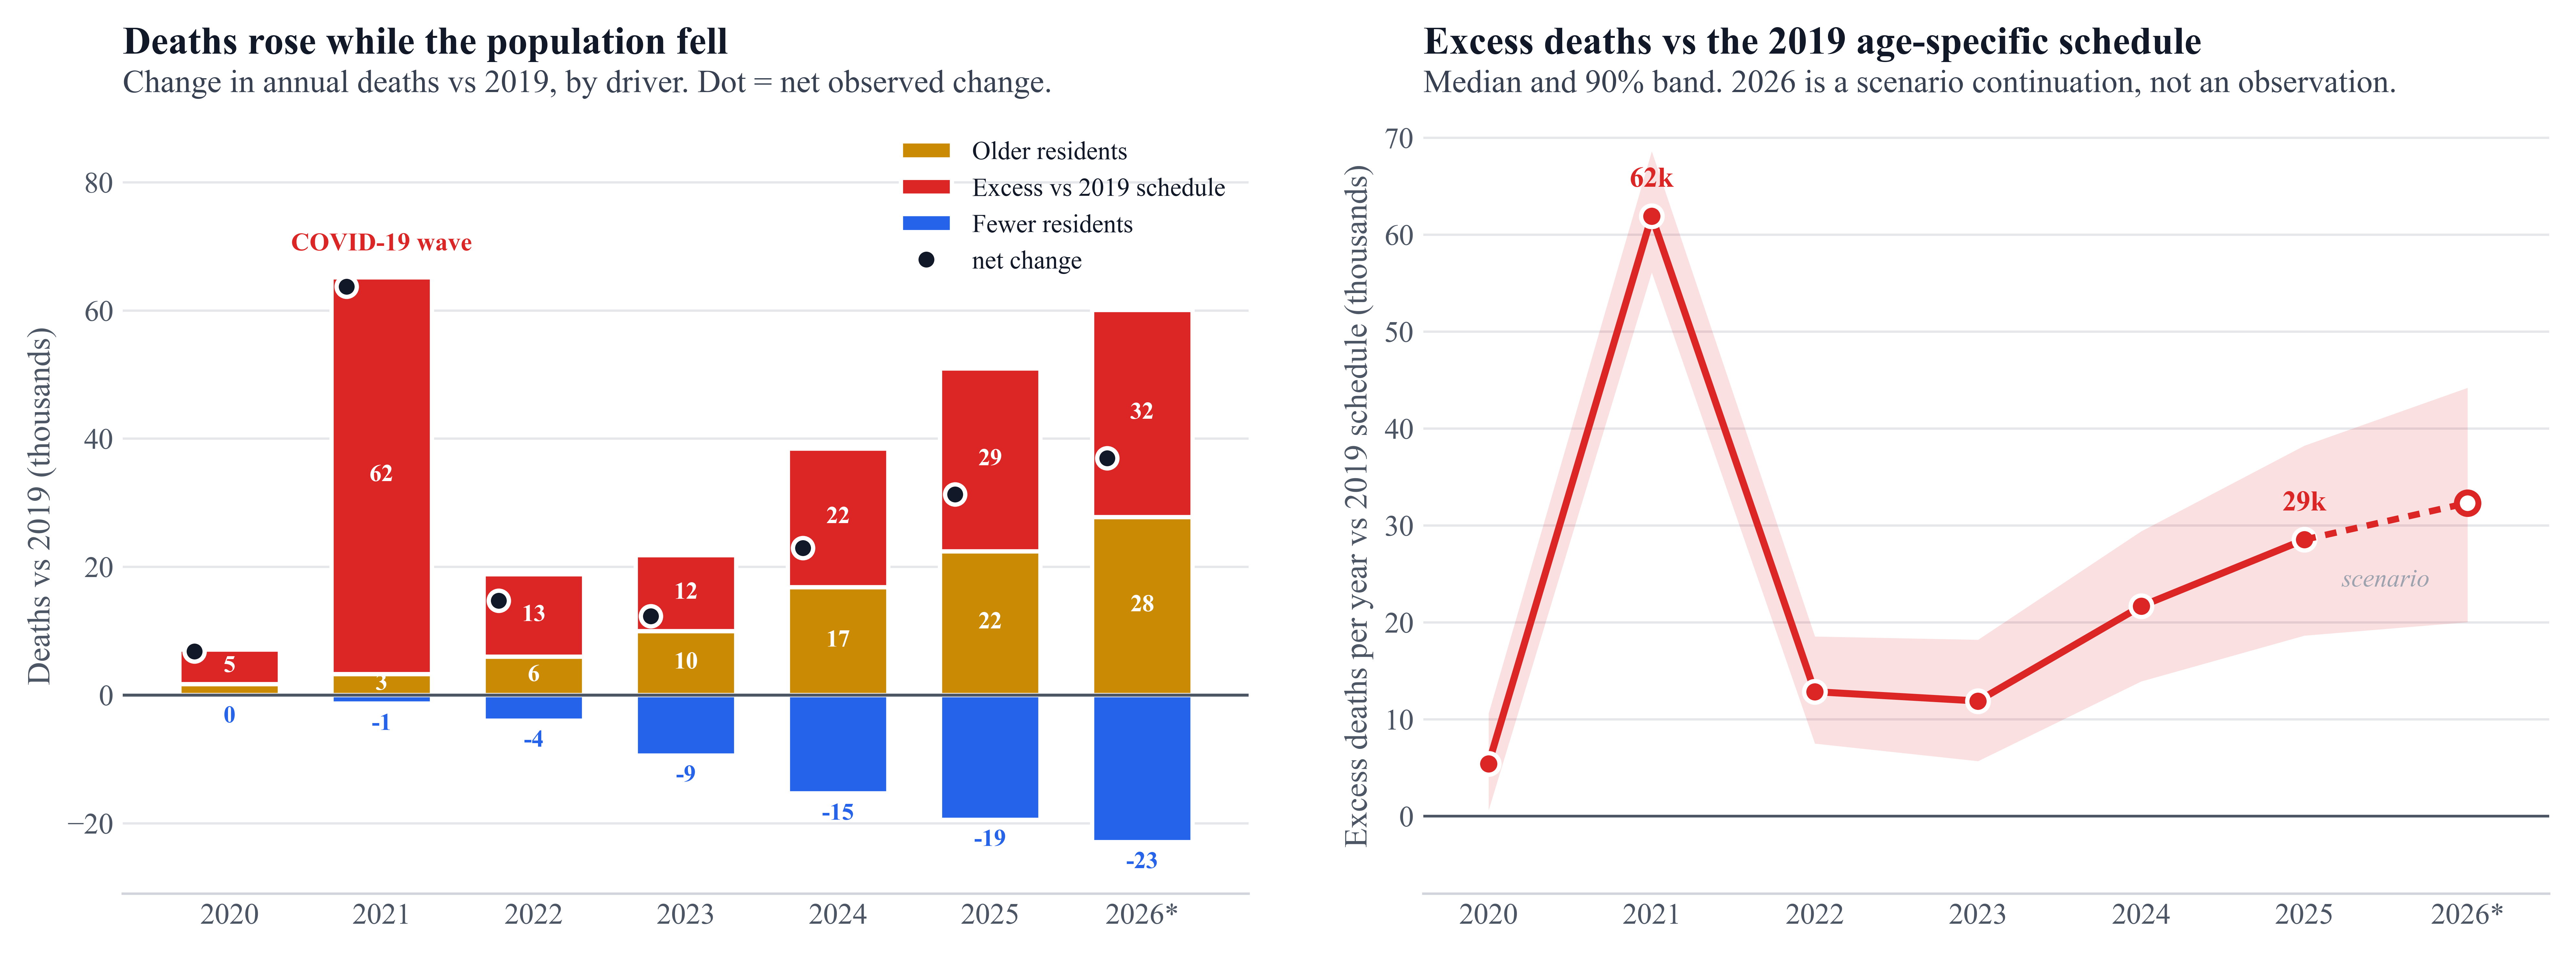
\includegraphics[width=\linewidth]{f14_atribuible.png}
\caption{Why deaths rose while the population fell.
Left: change in annual deaths versus 2019 decomposed into population size, ageing, and rate deterioration; the dot is the net observed change including estimated unregistered deaths.
Right: excess deaths against the 2019 schedule, median and prior sensitivity range.
2026 is a scenario continuation, not an observation.
Bands are prior-predictive under the stated margins and share $D_{\mathrm{fac}}$ with the central scenario.}
\label{fig:attrib}
\end{figure}

\subsection{Projected population}

Sources that do not purge emigrants (electoral roll, MINSAP health denominator) sit high and function as soft ceilings.
Exit-correcting constructs (housing occupancy $\sim$8.7~M; Albizu-Campos 8.0--8.6~M) sit near the central scenario but share migration-critique assumptions with this study; they are not independent censuses.
The official 9.43~M sits between the two families (Figure~\ref{fig:tri}).
Voter turnout fell sharply between 2018 and 2023; that pattern is compatible with physical absence but also with abstention, logistics, and political factors, and is \emph{not} used as a person count.

\begin{figure}[!htbp]
\centering
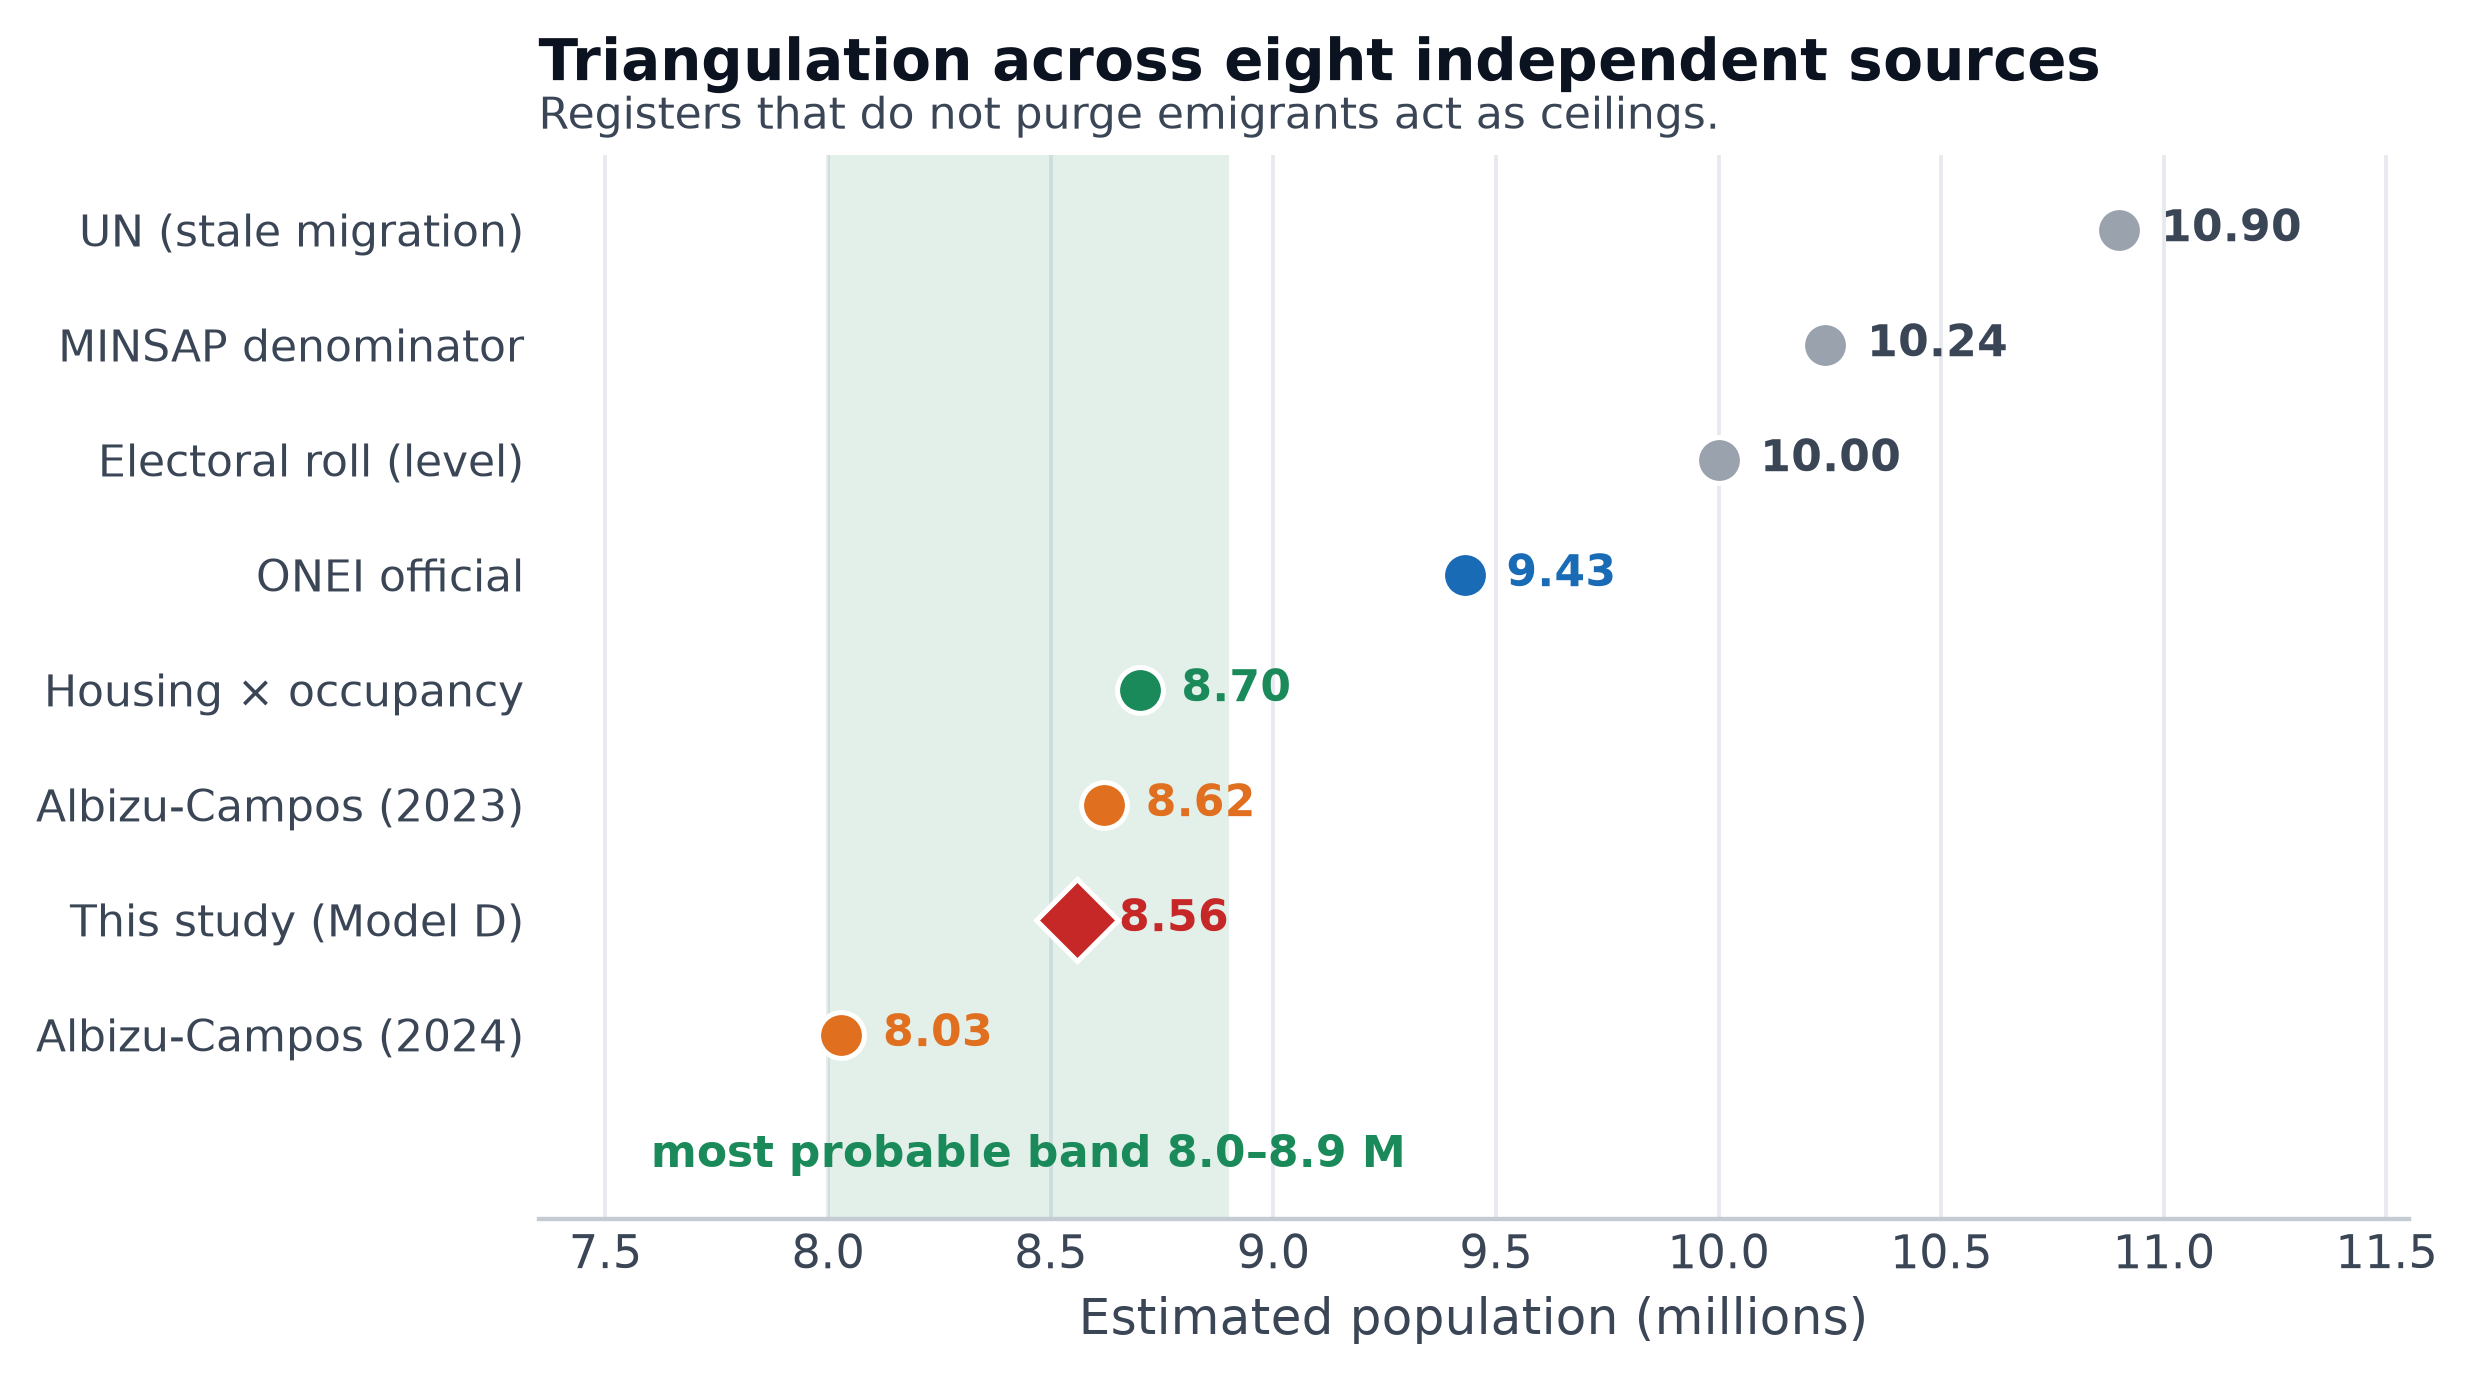
\includegraphics[width=0.95\linewidth]{f7_triangulacion.png}
\caption{Triangulation of end-2025 population levels.
the central scenario is the study estimand (not a validator); Albizu/housing are soft, assumption-laden anchors.}
\label{fig:tri}
\end{figure}

Table~\ref{tab:models} summarizes the three scenarios.
The primary uncertainty statement is the across-scenario envelope: against the official end-2021 stock of 11.11~million, the gap by end-2025 spans \textbf{1.97--2.79~million}, or \textbf{17.8--25.1\%}.
The central scenario places living population at \textbf{8.58~million} (gap \textbf{2.53~million}, \textbf{22.8\%}) against 9.43~million officially, with the floor at 9.14~million and the upper stress case at 8.32~million.
Emigration accounts for about \textbf{92\%} of the central gap once the pre-2021 backlog is counted alongside the 2022--2025 flow; within the flow alone it is $\sim$91\%.
The end-2026 continuation places the central scenario near \textbf{8.29~million} (envelope 8.02--8.84~million).
Because there is now a single base, the headline has a single form: between roughly one in six and one in four of the officially counted 2021 population is not there, with the central scenario near one in four\,--\,one in five.

\begin{table}[ht]
\centering
\caption{Three scenarios against one base: the official end-2021 stock (11{,}113{,}215).
Point estimates are closed form; within-scenario 90\% bands are prior sensitivity ranges over the stated margins. They are not confidence intervals, carry no coverage property, and no parameter in this paper is informed by a likelihood.
Earlier versions carried five prior sets; a crisis-adjusted variant (within 0.02~M of the central path) and a vital-reconstruction companion have been retired.}
\label{tab:models}
\begin{tabular}{lrrrr}
\toprule
Scenario & Gap (M) & Gap \% & Pop.\ end-2025 (M) & Pop.\ end-2026 (M) \\
\midrule
\textit{Null: ONEI at face value} & \textit{1.68} & \textit{15.1} & \textit{9.43} & \textit{9.14} \\
Conservative & 1.97 & 17.8 & 9.14 & 8.84 \\
\textbf{Crisis-adjusted central} & \textbf{2.53} & \textbf{22.8} & \textbf{8.58} & \textbf{8.29} \\
Upper stress & 2.79 & 25.1 & 8.32 & 8.02 \\
\midrule
\textit{Envelope (excl.\ null)} & \textit{1.97--2.79} & \textit{17.8--25.1} & \textit{8.32--9.14} & \textit{8.02--8.84} \\
\bottomrule
\end{tabular}
\end{table}

\begin{figure}[!htbp]
\centering
\begin{subfigure}[t]{0.495\linewidth}
\centering
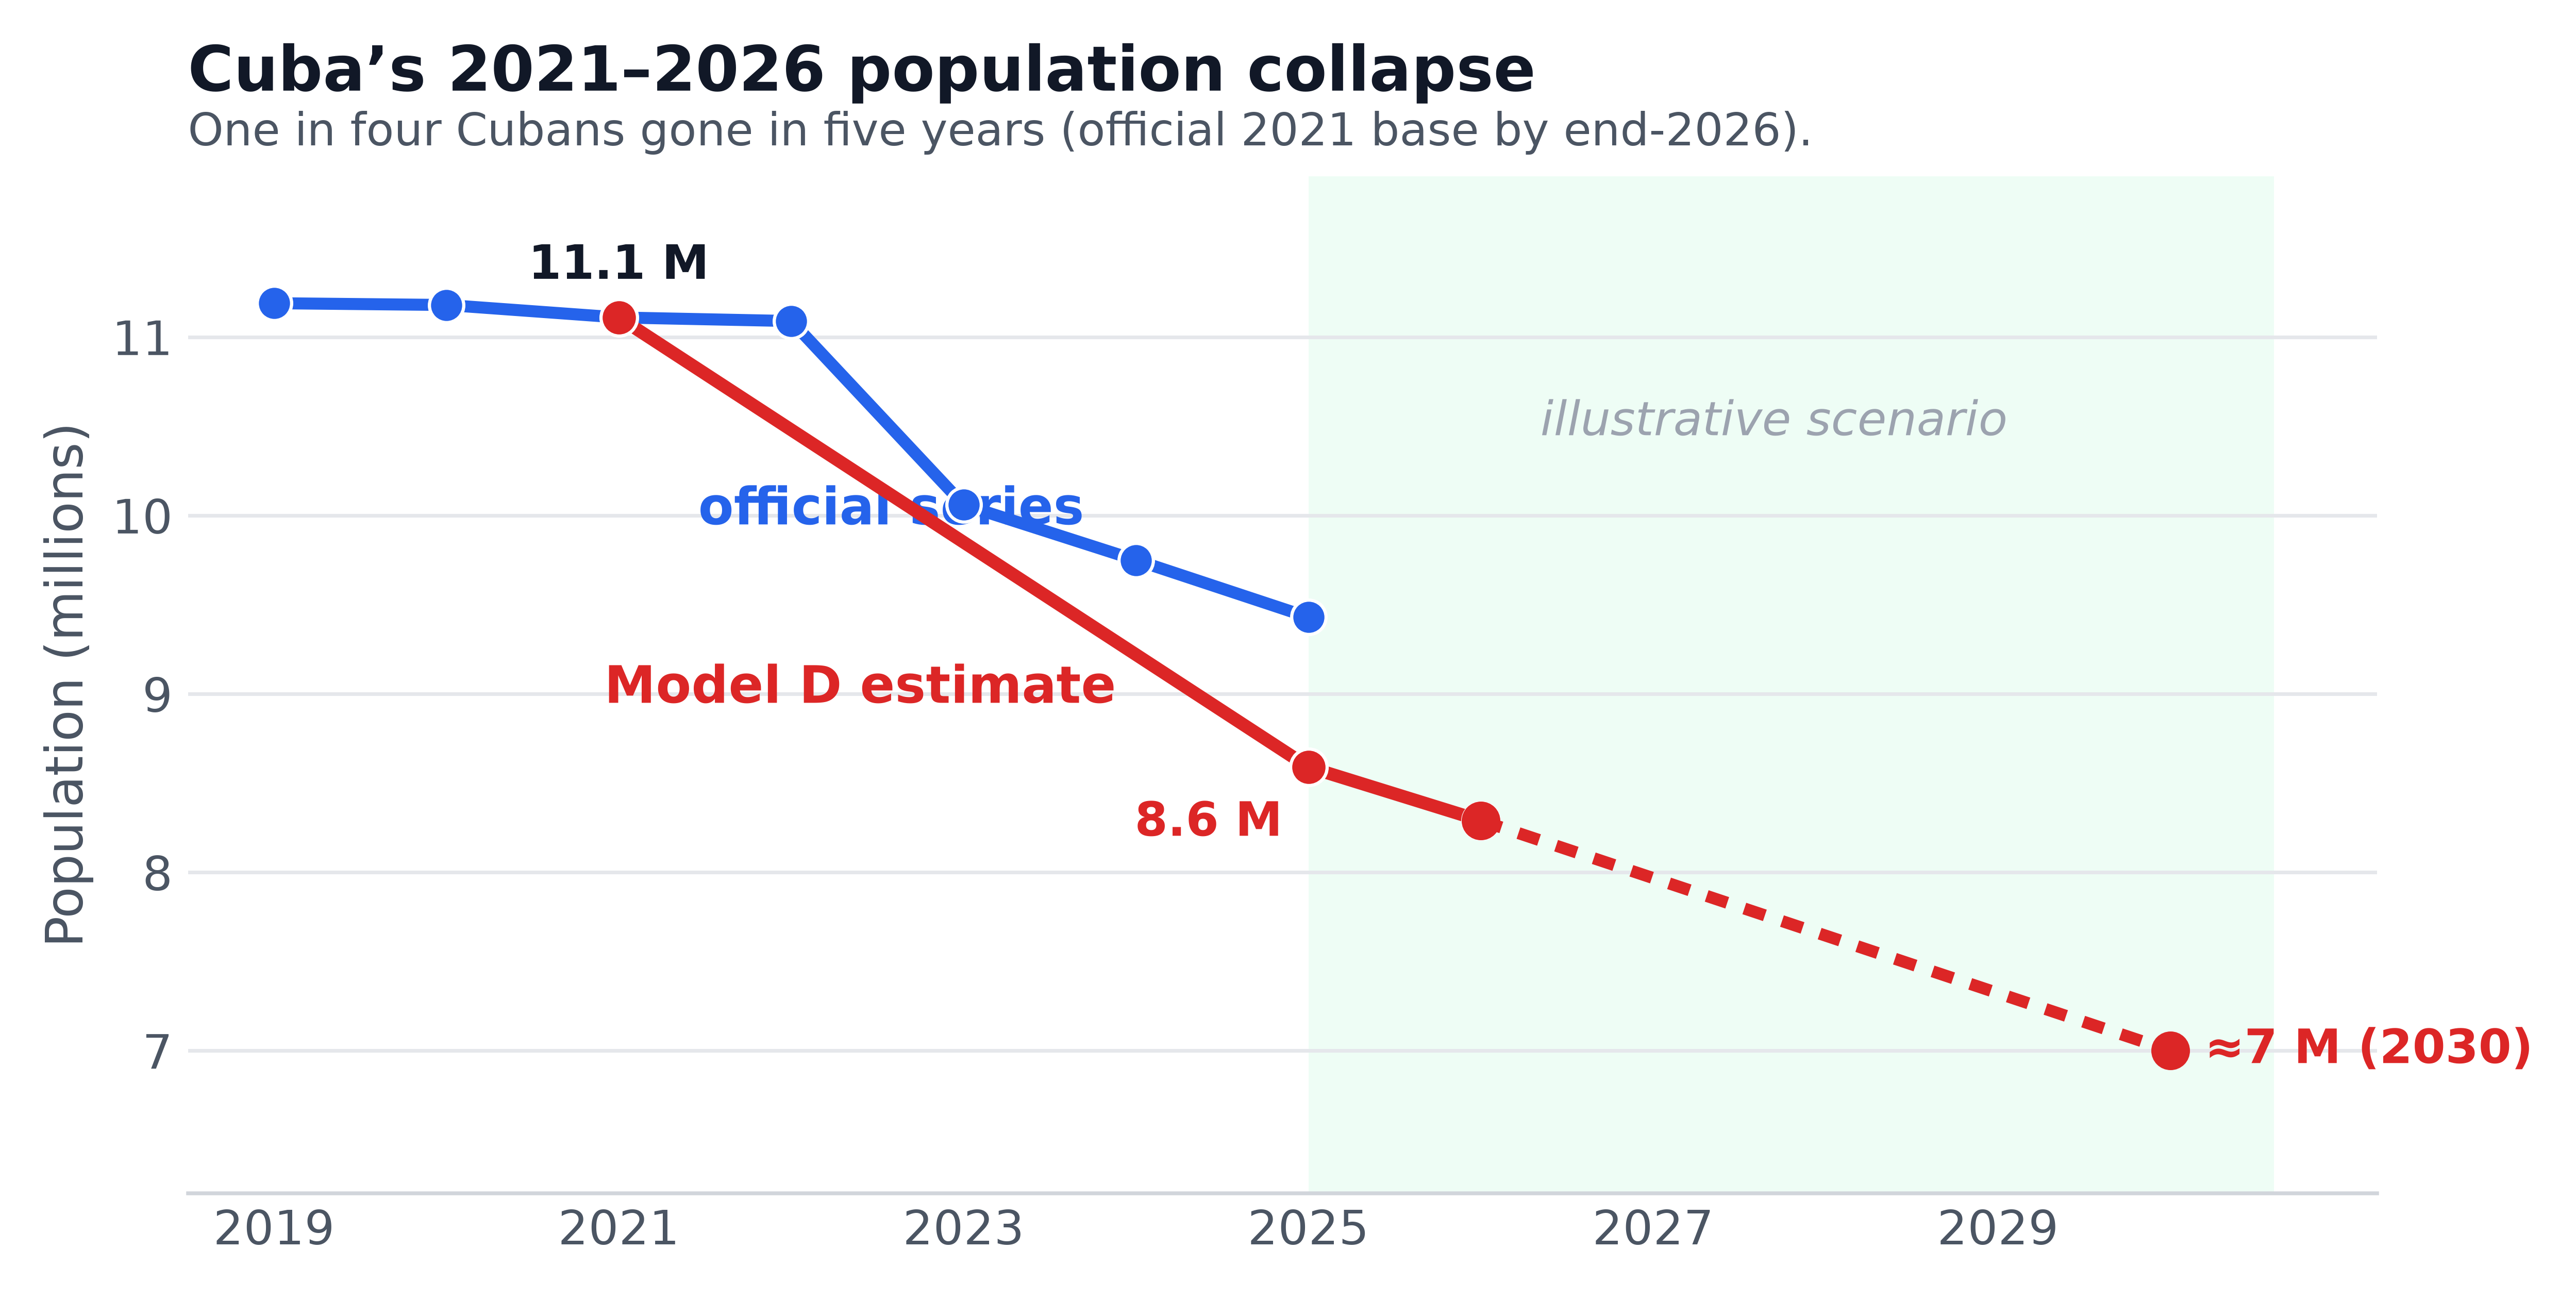
\includegraphics[width=\linewidth]{f1_poblacion.png}
\caption{Official versus scenario living population, 2021--2030 (the central scenario illustrative path in red; post-2026 segment is a non-probabilistic trend scenario).}
\label{fig:pop}
\end{subfigure}\hfill
\begin{subfigure}[t]{0.495\linewidth}
\centering
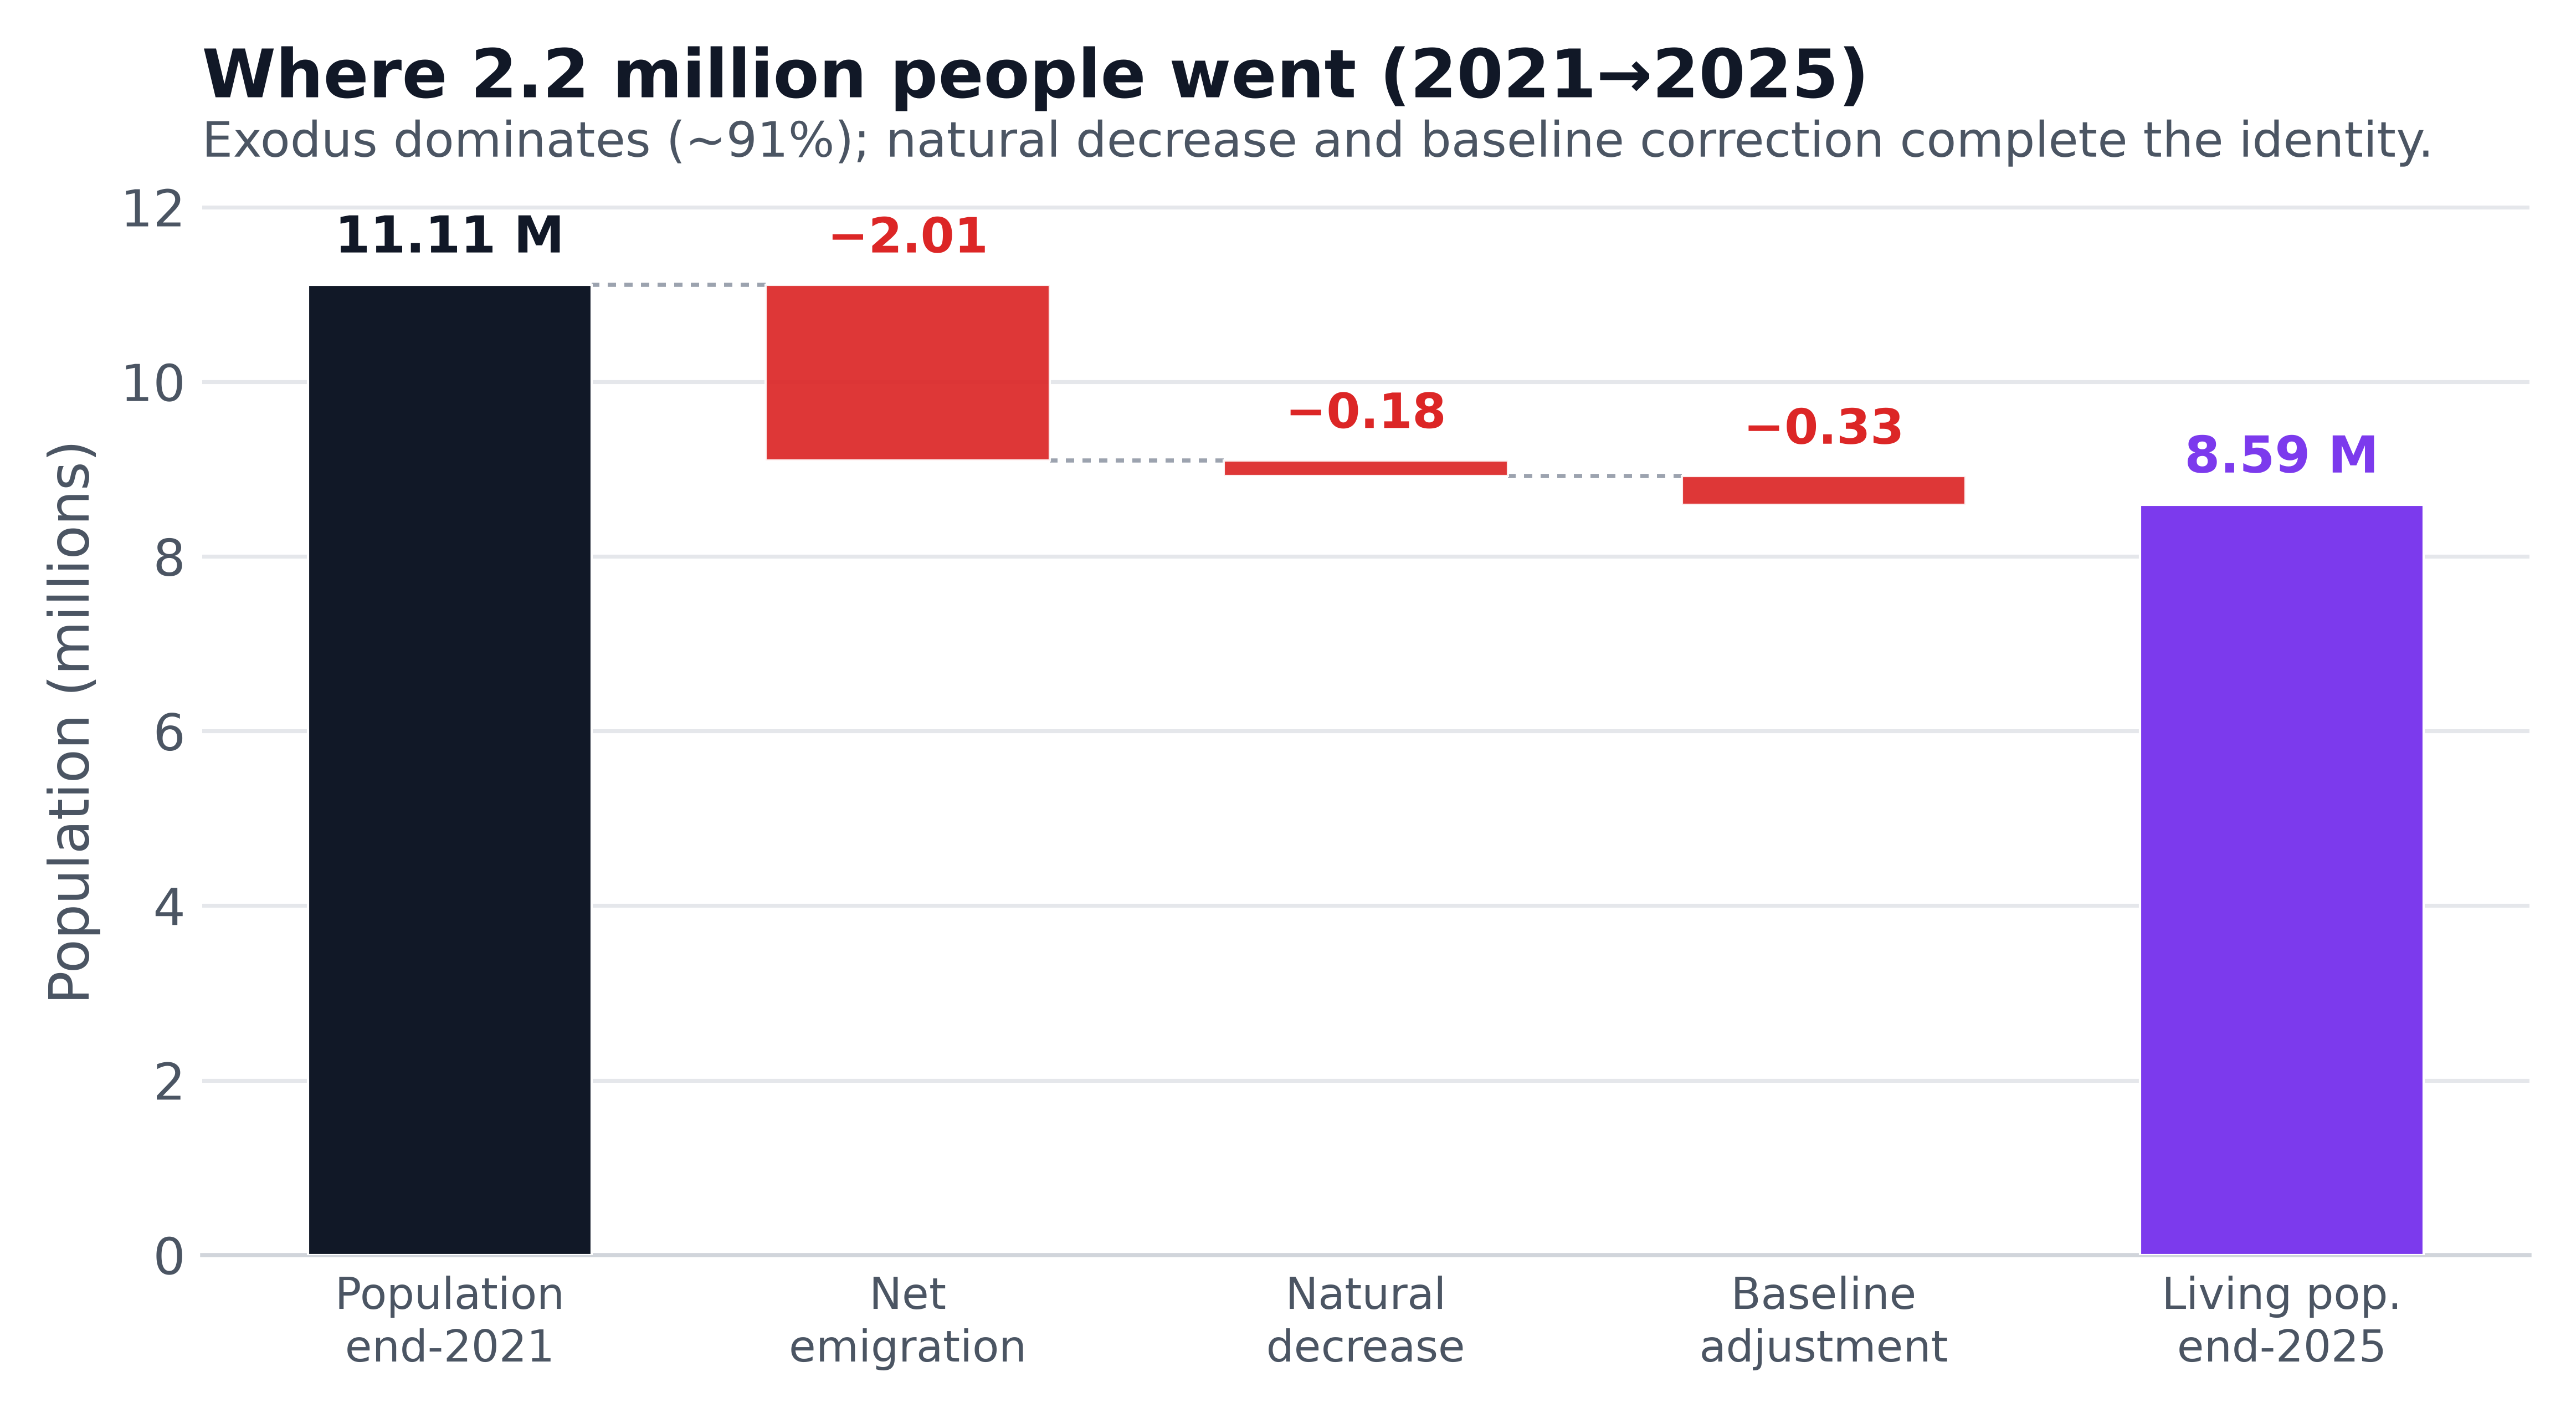
\includegraphics[width=\linewidth]{f3_cascada.png}
\caption{Accounting decomposition under the central scenario medians (2021--2025); illustrative scenario, not identified attribution.}
\label{fig:cascade}
\end{subfigure}
\caption{Headline population path and accounting decomposition.}
\label{fig:headline}
\end{figure}

Regionally, Latin America and the Caribbean still grow ($\sim$+$0.7\%$ per year; Table~\ref{tab:region}, UN WPP / CEPAL approximations).
Cuba shows net population loss of about $-$3.3\% annually on recent official-path comparisons.
Among peacetime emigration-driven contractions, Venezuela is the closest regional peer (Table~\ref{tab:hist}); disaster-driven cases are not treated as peers.
By \textbf{end-2026}, the central continuation implies about 300{,}000 further loss: living population near \textbf{8.29~million} (across-scenario band 8.02--8.84~M).
By end-2026 the upper scenario reaches a gap of $\sim$3.1~million; the central scenario $\sim$2.8~million ($\sim$25\%).
Illustrative trend paths toward $\sim$7~million by 2030 (Figure~\ref{fig:pop}, post-2026 segment) are scenarios only.

\begin{table}[ht]
\centering
\caption{Cuba versus selected peacetime emigration-driven contractions.
Cuba row uses the central scenario against the official 2021 base and therefore includes a pre-2021 register correction ($U_0$) plus ONEI's own 2023 backlog catch-up; it is a stock discrepancy, not a 2021--25 flow, and is not like-for-like with the comparators, which are population losses. Comparators are approximate and not window-harmonised. Puerto Rico row confounded by hurricane disaster.}
\label{tab:hist}
\begin{tabular}{lrrr}
\toprule
Case & Cum.\ loss & Approx.\ annual & Dominant engine \\
\midrule
Venezuela 2013--24 & $\sim$25\% & 1--3\% & emigration \\
Puerto Rico post-2017 (Mar{\'i}a era) & large net exit & --- & emigration + disaster \\
Cuba 2021--25 (central) & $\sim$22.8\% (official base) & $\sim$3--5\% & emigration + internal \\
\bottomrule
\end{tabular}
\end{table}

\begin{table}[ht]
\centering
\caption{Annual population growth: Cuba versus the region (approximate; UN WPP 2024 revision and CEPAL, rounded).}
\label{tab:region}
\begin{tabular}{lr}
\toprule
Country / region & Annual growth \\
\midrule
Guatemala & $+1.7\%$ \\
Bolivia & $+1.4\%$ \\
Dominican Republic & $+1.0\%$ \\
Mexico & $+0.8\%$ \\
Colombia & $+0.7\%$ \\
\textit{Latin America \& Caribbean} & $+0.7\%$ \\
Brazil & $+0.4\%$ \\
Chile & $+0.3\%$ \\
Uruguay & $+0.1\%$ \\
Venezuela & $\approx 0\%$ (after $\sim$25\% loss 2013--24) \\
Cuba & $-3.3\%$ \\
\bottomrule
\end{tabular}
\end{table}

\section{Discussion}

\subsection{Migration}



The one documented instance of the death register being revised downward is instructive.
We use the published figure, but the pre-revision total would raise 2022 excess mortality from $\sim$12{,}700 to $\sim$21{,}900 and the 2022--2025 post-pandemic total from $\sim$74{,}800 to $\sim$84{,}100.
This is the empirical anchor for how much slack the register demonstrably has: 7.5\% in a single year, just below the 9\% cap on $D_{\mathrm{fac}}$, which is why that cap is retained rather than raised.
It bounds the question from observation rather than from prior belief, and it cuts both ways---a register that can shed 8{,}951 deaths without explanation is not fully trustworthy, but one that published a 54\% single-year surge in 2021 (109{,}080 to 167{,}645) is also not one that hides at scale.

ONEI's declared 2022 net migration ($+$991) is inconsistent with hundreds of thousands of U.S.\ Cuban arrivals that year at any plausible encounter-to-emigrant conversion (encounters are not unique net emigrants 1:1).
Much of the exodus is booked in a single 2023 revision, consistent with a lagged register catch-up recorded within one year.
Even after that revision, 2024--2025 net balances remain only slightly above U.S.-only recorded entries, while the 2025 balance admits 317{,}320 gross external emigrations (net $-$245{,}264): a shortfall against the multi-destination floor, though the 2025 balance is internally consistent.
This paper therefore treats the official headcount as a ceiling and contrasts it with exit-correcting sources (Figure~\ref{fig:tri}).

Taken together: against the official end-2021 stock, the gap by end-2025 lies between 1.97 and 2.79~million, or 17.8--25.1\% (the primary statement).
Under the central scenario, living population is near 8.58~million at end-2025 rather than the official 9.43~million, a gap of 2.53~million (22.8\%), about 92\% of it emigration; the ONEI-anchored floor sits at 9.14~million.
By end-2026 the central continuation is near 8.29~million, taking the gap to roughly one in four.
Alongside that headcount---of whose 2.53~million gap 1.68~million is ONEI's own published decline and 0.85~million this paper's correction---excess mortality against the 2019 schedule runs at $\sim$28{,}500 deaths a year at 2025 levels and $\sim$74{,}800 cumulatively over 2022--2025, a toll larger than what ageing alone explains and about a third below what the crude bridge previously implied for 2024--2025.
A 2026 census conducted under standard practice would be informative; the working end-2026 scenario band is 7.9--8.9~million rather than the 10.9~million World Population Prospects path under still-low net-emigration assumptions~\citep{un_wpp}.


\subsection{Health-system deterioration}

The two engines meet in the mortality decomposition, and reading it correctly matters.
Emigration removes working-age adults, which raises the elderly share, which raises deaths even with an unchanged health system: that is the $\sim$22{,}400 additional deaths a year the ageing term measures.
How much of that ageing is migration-induced is \emph{not} identified here---the term is computed from the observed ONEI age structure, and Cuba's fertility transition was already generating ageing decades before the crisis---so it should be read as ageing from all causes combined, of which selective exit is one.
On top of it sits a rate deterioration of $\sim$28{,}500 deaths a year that ageing does not explain, concentrated in 2024--2025 and still rising in the 2026 scenario.
The policy-relevant asymmetry is that emigration can reverse, whereas neither those deaths nor the births that did not occur can.
Two properties make the excess estimate more robust than the population scenarios it sits beside: it does not depend on resolving the migration dispute, because the elderly count is held approximately fixed and $E_t$ therefore barely moves between the official and the central scenario stocks; and it is insensitive to the anchor's \emph{level}, which 2017--2019 sensitivity leaves essentially unchanged at ages 60+ (it is \emph{not} insensitive to the anchor's trend, which is the dominant uncertainty above).
It remains conditional on registered deaths being close to complete---an assumption the infant-mortality sentinel makes plausible for institutional deaths but does not establish, and which the $D_{\mathrm{fac}}$ prior is meant to absorb rather than resolve.
Its principal weakness is the opposite of the population models': the mechanism is unidentified.
Blackouts, fuel-driven ambulance and dialysis failures, drug shortages, delayed oncology, and the 2025--2026 arbovirus waves are all plausible pathways, and none is separately estimated here; the estimate is an association with the crisis period, not a cause-of-death attribution.
WFP food-insecurity and anaemia indicators, and the fall in agricultural GDP, are discussed only as \emph{contextual} amplifying pathways~\citep{wfp_cuba}; they do not enter $D_{\mathrm{fac}}$ or the decomposition~\citep{karlinsky2021,msemburi2023}.


\subsection{Projected population}

The central scenario is retained because the IMR consistency check shrinks the need for large hidden-death multipliers and focuses residual uncertainty on migration~\citep{pagegarcia2020,modeld}.
It is not an identified point estimate: absolute loss remains $\sim$91\% migratory under the central scenario's priors, and $U_0$ with $M>1$ can share a common outdated-register defect.
Within-scenario intervals look falsely precise relative to the across-scenario envelope---the envelope should lead.
The scientific lead is the 0.85~million by which the central scenario falls below ONEI's own end-2025 figure. The 2.53~million (22.8\%) gap against the official 2021 base is the sum of that correction and the 1.68~million ONEI has itself already published; the two must not be quoted interchangeably.
Exit is age- and sex-selective; it ages the island and structurally depresses fertility~\citep{coleman2006,diazbriquets2014,lee2014}.
The natural balance, positive in 2019, fell to $-$68{,}150 in 2025.

\section{Disclaimers}

\textbf{Limitations.}
There has been no census since 2012; ONEI's $\sim$24-month emigration rule lags recent exits; destination microdata are incomplete; U.S.\ ``settled'' administrative totals are not ACS stock; housing-occupancy assumptions are fragile; ageing sketches are not cohort-component projections; life expectancy re-expresses mortality; 2026--2030 paths are scenarios.
$U_0$ and $M$ can double-count register lag; destination encounter ceilings can inflate unique persons; within-scenario intervals give false precision relative to structural uncertainty.
The mortality decomposition uses four age groups because that is the finest set ONEI 3.15 and 3.3 share; both ONEI 3.15 and 3.3 stop at 2022, so the 2023--2026 age structure is a cohort projection rather than an observation, and within-65+ composition after 2022 enters as a residual drift parameter.
Its 2019 anchor assumes no counterfactual post-2019 improvement in Cuban mortality, and it shares $D_{\mathrm{fac}}$ with the central scenario, so it is not independent of the headcount scenario.
Excess deaths against the 2019 schedule are an association with the crisis period, not a cause-of-death attribution.
Food-insecurity indicators are contextual only.

The pre-crisis age-standardised series cannot be fitted on a complete window: ONEI 3.15 panels for 2009--2012 parse to roughly half the true death totals and are rejected by a reader guard, so the trend rests on 10 non-contiguous years (or 7 contiguous ones, which give a trend nearly three times larger). On either window the slope is statistically indistinguishable from zero, so no pre-crisis trend is available to fit, and the flat anchor should be read as a convention.
The dominant uncertainty in the mortality estimand is the choice of counterfactual, not anything inside the simulation, and it is reported separately rather than folded into the range.

\textbf{Status.}
This is a preprint and has not been peer reviewed.
The three scenarios are prior narratives, not identified estimators of a unique living population, and reported bands are prior-predictive spreads rather than sampling error from data.

\textbf{Data and code availability.}
ONEI tables and a machine-readable claim sheet are in the public repository
\url{https://github.com/ypriverol/cubascience} under \texttt{demographics/}.
Interactive companion: \url{https://ypriverol.github.io/cubascience/demographics/}.
Monte Carlo scripts (\texttt{scripts/model\_*.py}) and the mortality decomposition
(\texttt{scripts/attributable\_mortality.py}) write summaries to \texttt{artifacts/}.
Supplementary PDF: \texttt{manuscript/en/cuba-depopulation-2021-2026-supplement.pdf}~\citep{modele_supp}.
Third-party literature is cited, not redistributed.

\textbf{Competing interests.}
None declared.

\FloatBarrier
\bibliographystyle{plainnat}
\bibliography{refs}

\end{document}
